\begin{figure*}[ht!]
\centering
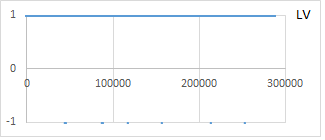
\includegraphics[width=0.32\linewidth]{tex-figures/loops/live.png}
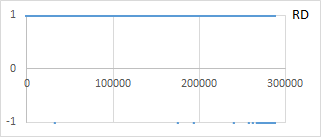
\includegraphics[width=0.32\linewidth]{tex-figures/loops/reach-def.png}
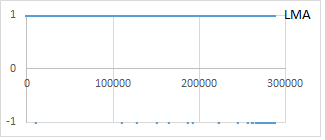
\includegraphics[width=0.32\linewidth]{tex-figures/loops/lma.png}
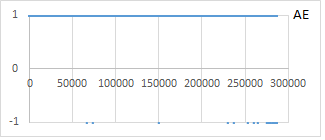
\includegraphics[width=0.32\linewidth]{tex-figures/loops/avail.png}
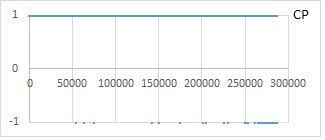
\includegraphics[width=0.32\linewidth]{tex-figures/loops/copy.png}
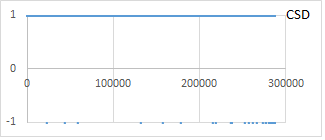
\includegraphics[width=0.32\linewidth]{tex-figures/loops/csd.png}
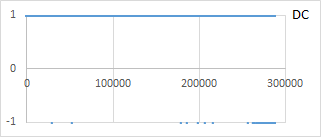
\includegraphics[width=0.32\linewidth]{tex-figures/loops/dead.png}
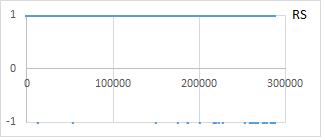
\includegraphics[width=0.32\linewidth]{tex-figures/loops/fileopenclose.png}
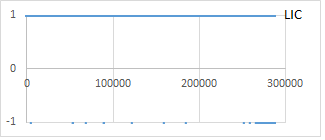
\includegraphics[width=0.32\linewidth]{tex-figures/loops/LIC.png}
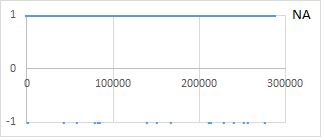
\includegraphics[width=0.32\linewidth]{tex-figures/loops/nullness.png}
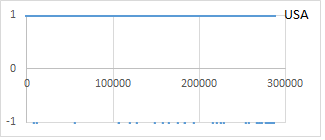
\includegraphics[width=0.32\linewidth]{tex-figures/loops/usa.png}
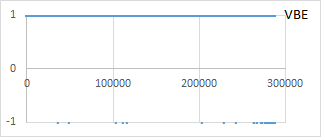
\includegraphics[width=0.32\linewidth]{tex-figures/loops/vbe.png}
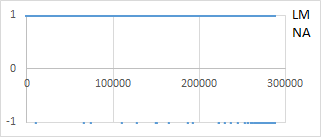
\includegraphics[width=0.32\linewidth]{tex-figures/loops/lmna.png}
\caption[Binary chart for analysis that has loop sensitive traversal. 1 indicates correct traversal strategy prediction and -1 indicates mis-prediction.]{Binary chart for analysis that has loop sensitive traversal. 1 indicates correct traversal strategy prediction and -1 indicates mis-prediction.}
\label{fig:loops}
\end{figure*}
